\documentclass{article}
\usepackage[letterpaper,top=2cm,bottom=2cm,left=3cm,right=3cm,marginparwidth=1.75cm]{geometry}
\usepackage{amsmath}
\usepackage{amssymb}
\usepackage{tikz}
\usepackage{pgfplots}

\newcommand{\solution}{\textbf{Solution: }}
\newcommand{\der}[3][]{\frac{d^{#1} #2}{d #3^{#1}}}
\newcommand{\pder}[3][]{\frac{\partial^{#1} #2}{\partial #3^{#1}}}
\newcommand{\inv}{^{-1}}

\pgfplotsset{compat = newest}
%\includeonly{Section1-3}

\title{Math 20D HW1}
\author{Merrick Qiu}


\begin{document}
\maketitle
\newpage

\subsection*{Section 1.1}
Classify the following as an ODE/PDE, give the order,
and indicate the independent and dependent variables.
If the equation is an ODE, indicate whether the equation is linear or nonlinear.\\
\textbf{Problem 2}
\[
    \der[2]{y}{x} - 2x\der{y}{x} + 2y = 0
\]
\begin{enumerate}
    \item Linear ODE with respect to $x$
    \item Order 2
    \item Independent variables: $x$
    \item Dependent variables: $y$
\end{enumerate}
\textbf{Problem 3}
\[
    \der{y}{x} = \frac{y(2-3x)}{x(1-3y)}
\]
\begin{enumerate}
    \item Nonlinear ODE with respect to $x$
    \item Order 1
    \item Independent variables: $x$
    \item Dependent variables: $y$
\end{enumerate}
\textbf{Problem 4}
\[
    \pder[2]{u}{x} + \pder[2]{u}{y} = 0
\]
\begin{enumerate}
    \item PDE 
    \item Order 2
    \item Independent variables: $x$, $y$
    \item Dependent variables: $u$
\end{enumerate}
\textbf{Problem 6}
\[
    \der{x}{t} = k(4-x)(1-x)
\]
\begin{enumerate}
    \item Nonlinear ODE with respect to $t$
    \item Order 1
    \item Independent variables: $t$
    \item Dependent variables: $x$
\end{enumerate}
\textbf{Problem 8}
\[
    \sqrt{1-y}\der[2]{y}{x} + 2x\der{y}{x} = 0
\]
\begin{enumerate}
    \item Nonlinear ODE with respect to $x$
    \item Order 2
    \item Independent variables: $x$
    \item Dependent variables: $y$
\end{enumerate}
\textbf{Problem 16}
Write the differential equation that fits the description:
The rate of change of $A$ at time $t$ is proportional
to the square of $A$ at time $t$.

\solution
\[
    \der{A}{t} = kA^2
\]
\newpage
\subsection*{Section 1.2}
\textbf{Problem 1}
\begin{enumerate}
    \item Show that $\phi(x) = x^2$ is a solution to 
        \[
            x\der{y}{x} = 2y
        \]
    \item Show that $\phi(x) = e^x-x$ is a solution to 
        \[
            \der{y}{x} + y^2 = e^{2x} + (1-2x)e^x + x^2 -1
        \]
    \item Show that $\phi(x) = x^2 - x\inv$ is a solution to
        \[
            x^2 \der[2]{y}{x} = 2y
        \]
\end{enumerate}
\solution
\begin{enumerate}
    \item Substituting $\phi(x)$ in for $y$ yields an equation 
        that is true for all $x \in (-\infty, \infty)$.
        \[
            x\der{y}{x} = 2y
            \implies x(2x) = 2(x^2)
            \implies 2x^2 = 2x^2
        \]
    \item Substituting $\phi(x)$ in for $y$ yields an equation
        that is true for all $x \in (-\infty, \infty)$.
        \begin{align*}
            \der{y}{x} + y^2 = e^{2x} + (1-2x)e^x + x^2 -1
            &\implies (e^x-1) + (e^x-x)^2 = e^{2x} + (1-2x)e^x + x^2 -1 \\
            &\implies (e^x-1) + (e^x-x)^2 = (e^x-x)^2 + e^x - 1 \\ 
            &\implies (e^x-1) + (e^x-x)^2 = (e^x-1) + (e^x-x)^2
        \end{align*}
    \item Substituting $\phi(x)$ in for $y$ yields an equation
        that is true for all $x \in (0, \infty)$.
        \begin{align*}
            x^2 \der[2]{y}{x} = 2y
            &\implies x^2 (2- 2x^{-3}) = 2(x^2-x\inv) \\
            &\implies 2x^2 - 2x\inv = 2x^2-2x\inv
        \end{align*}
\end{enumerate}
\textbf{Problem 4}

Determine if $x = 2\cos t - 3\sin t$ is a solution to $x''+ x = 0$ \\
\solution
It is a solution since 
\begin{align*}
    x''+ x = 0
    &\implies (-2\cos t + 3\sin t) + (2\cos t - 3\sin t) = 0 \\
    &\implies 0 = 0
\end{align*}
\textbf{Problem 10}

Determine if $y-\ln(y) = x^2+1$ is an implicit solution to 
$\der{y}{x} = \frac{2xy}{y-1}$ \\
\solution 
It is a solution since
\begin{align*}
    y-\ln(y) = x^2+1
    &\implies \der{y}{x} - \frac{1}{y}\der{y}{x} = 2x \\
    &\implies \der{y}{x} (1-\frac{1}{y}) = 2x \\ 
    &\implies \der{y}{x} (\frac{y-1}{y}) = 2x \\ 
    &\implies \der{y}{x} = \frac{2xy}{y-1}
\end{align*}
\textbf{Problem 22}

Verify that $\phi(x) = c_1e^x + c_2e^{-2x}$
is a solution to 
\[
    \der[2]{y}{x} + \der{y}{x} - 2y = 0
\]
and find $c_1$ and $c_2$ that satisfies
\begin{enumerate}
    \item $y(0) = 2$, $y'(0) = 1$
    \item $y(1) = 1$, $y'(1) = 0$
\end{enumerate} 
\solution 
Substituting in $\phi$ yields 
\begin{align*}
    \der[2]{y}{x} + \der{y}{x} - 2y = 0
    &\implies (c_1e^x + 4c_2e^{-2x}) + (c_1e^x - 2c_2e^{-2x}) - 2(c_1e^x + c_2e^{-2x}) = 0 \\
    &\implies 0 = 0
\end{align*}
\begin{enumerate}
    \item 
        \[
            \phi(0) = 2 
            \implies c_1e^0 + c_2e^0 = 2
            \implies c_1 + c_2 = 2
        \]
        \[
            \phi'(0) = 1
            \implies c_1e^0 - 2c_2e^0 = 1
            \implies c_1 - 2c_2 = 1
        \]
        Solving this system of equations yields 
        $c_1 = \frac{5}{3}$ and $c_2 = \frac{1}{3}$.
    \item 
        \[
            \phi(1) = 1
            \implies c_1e^1 + c_2e^{-2} = 1
            \implies ec_1 + e^{-2}c_2 = 1
        \]
        \[
            \phi'(1) = 0
            \implies c_1e^1 - 2c_2e^{-2} = 0
            \implies ec_1 - 2 e^{-2}c_2 = 0
        \]
        Solving this system of equations yields 
        $c_1 = \frac{2}{3e}$ and $c_2 = \frac{e^2}{3}$.
\end{enumerate}
\textbf{Problem 24}

Does $\der{y}{t} - ty = \sin^2 t$ with $y(\pi)=5$
have a unique solution? \\
\solution
$f(t,y) = ty + \sin^2 t$ is always continuous and 
$\pder{f}{y} = t$ is also always continuous so 
the differential equation has a unique solution.

\textbf{Problem 26}

Does $\der{x}{t} + \cos x = \sin t$ with $x(\pi) = 0$
have a unique solution? \\
\solution 
$f(t,x) = \sin t-\cos x$ is always continuous and 
$\pder{f}{x} = \sin x$ is also always continuous so 
the differential equation has a unique solution.

\textbf{Problem 28}

Does $\der{y}{x} = 3x - \sqrt[3]{y-1}$ with $y(2) = 1$
have a unique solution? \\
\solution 
$f(x, y) = 3x - \sqrt[3]{y-1}$ is always continuous but
$\pder{f}{y} = -\frac{1}{3}(y-1)^{-\frac{2}{3}}$ 
is not continuous for $y_0 = 1$ so 
the theorem does not apply.

\newpage 
\subsection*{Section 1.3}
\textbf{Problem 2}

For $\der{y}{x} = 2x+y$,
\begin{enumerate}
    \item Find and sketch the solution through $(0,-2)$
    \item Sketch the solution through $(-1,3)$
    \item What can you say about the solution 
        as $x \to \infty$ and $x \to -\infty$?
\end{enumerate}

\solution
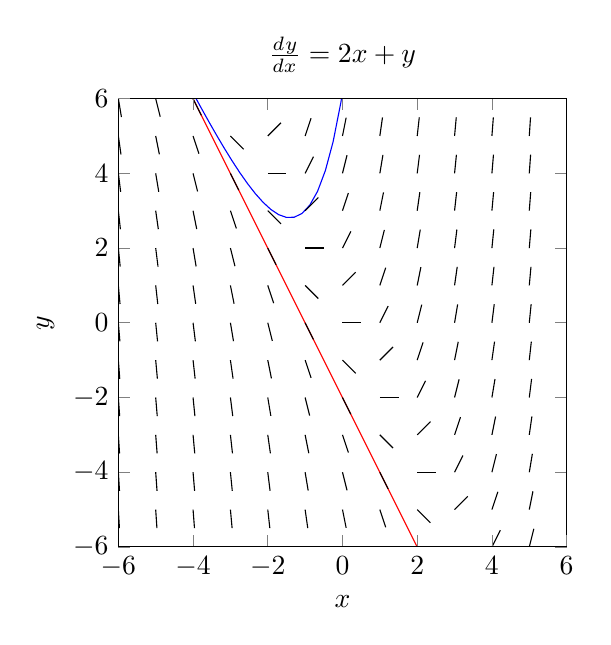
\begin{tikzpicture}
    \begin{axis}[
        xmin = -6, xmax = 6,
        ymin = -6, ymax = 6,
        zmin = 0, zmax = 1,
        axis equal image,
        view = {0}{90},
        title = {$\der{y}{x} = 2x+y$},
        xlabel = {$x$},
        ylabel = {$y$},
    ]
    \addplot[red, domain=-6:6]{-2*x-2};
    \addplot[blue, domain=-4:1]{3*e^(x+1)-2*x-2};
    \addplot3[
        quiver = {
            u = {1/sqrt(1+(2*x+y)^2)},
            v = {(2*x+y)/sqrt(1+(2*x+y)^2)},
            scale arrows = 0.5,
        },
        samples = 13,
        domain = -6:6,
        domain y = -6:6,
    ] {0};
    \end{axis}
\end{tikzpicture}

\begin{enumerate}
    \item The solution through $(0, -2)$ is shown by the red curve.
        The slope is
        \[
            \der{y}{x}|_{x=0} 
            = 2(0) + y 
            = y 
            = -2
        \]
        In order for the point to pass through $(0, -2)$, 
        the y-intercept must be $-2$.
        Therefore, the equation of the line is $y = -2x-2$.
    \item The solution through $(-1, 3)$ is shown by the blue curve.
    \item The solution goes to $\infty$ for both 
        $x \to \infty$ and $x \to -\infty$.
\end{enumerate}

\textbf{Problem 3}

For $\der{v}{t} = 1-\frac{v}{8}$, 
sketch the solutions for $v(0) = 5, 8, 15$
Why is $v=8$ the terminal velocity?

\solution

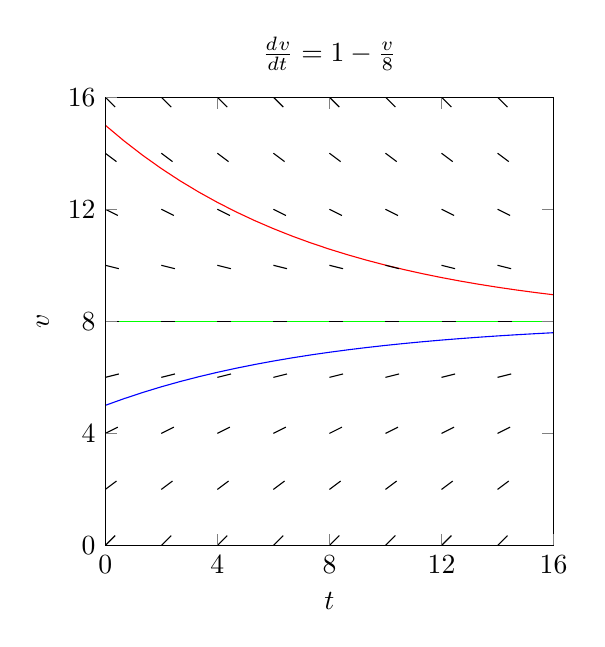
\begin{tikzpicture}
    \begin{axis}[
        xmin = 0, xmax = 16,
        ymin = 0, ymax = 16,
        zmin = 0, zmax = 1,
        axis equal image,
        view = {0}{90},
        title = {$\der{v}{t} = 1-\frac{v}{8}$},
        xlabel = {$t$},
        ylabel = {$v$},
        xtick = {0,4,8,12,16},
        xticklabels = {$0$,$4$,$8$,$12$,$16$},
        ytick = {0,4,8,12,16},
        yticklabels = {$0$,$4$,$8$,$12$,$16$},
    ]
    \addplot[red, domain=0:16]{7*e^(-x/8)+8};
    \addplot[green, domain=0:16]{8};
    \addplot[blue, domain=0:16]{-3*e^(-x/8)+8};
    
    \addplot3[
        quiver = {
            u = {1/sqrt(1+(1-y/8)^2)},
            v = {(1-y/8)/sqrt(1+(1-y/8)^2)},
            scale arrows = 0.5,
        },
        samples = 9,
        domain = 0:16,
        domain y = 0:16,
    ] {0};
    \end{axis}
\end{tikzpicture}

The red curve is the solution for $y(0) = 15$,
the green curve is the solution for $y(0) = 8$,
and the blue curve is the solution for $y(0) = 5$.
8 is the terminal velocity because the velocity approaches 8
for all solutions. \\
\textbf{Problem 6}
Consider 
\[
    \der{y}{x} = x + \sin y
\]
\begin{enumerate}
    \item What is the slope at $(1, \frac{\pi}{2})$?
    \item Argue that the solution curve increases for $x>1$.
    \item Show that all solutions satisfy 
        \[
            \der[2]{y}{x} = 1 + x\cos y + \frac{1}{2} \sin 2y
        \]
    \item Prove that the curve through $(0, 0)$ has a relative minimum at $(0,0)$.
\end{enumerate}
\solution 
\begin{enumerate}
    \item The slope is zero.
    \[
        \der{y}{x} = x + \sin y = 1 + \sin \frac{\pi}{2} = 2
    \]
    \item $\sin y$ can be at minimum $-1$, so 
        $x + \sin y$ must be positive for $x > 1$.
    \item Using the chain rule 
        \begin{align*}
            \der[2]{y}{x} 
            &= 1 + \cos(y) \der{y}{x} \\
            &= 1 + \cos(y)(x + \sin y) \\
            &= 1 + x\cos y + \sin y \cos y \\
            &= 1 + x\cos y + \frac{1}{2} \sin 2y
        \end{align*}
    \item Since $\der{y}{x} = 0$ and $\der[2]{y}{x} = 1 > 0$
        at $(0,0)$, the curve has a relative minimum at this point.
\end{enumerate}
\textbf{Problem 8}
\[
    \der{x}{t} = t^3 - x^3
\]
\begin{enumerate}
    \item What is the velocity at $x=1$ and $t=2$?
    \item Show that the acceleration is
        \[
            \der[2]{x}{t} = 3t^2 - 3t^3x^2 + 3x^5
        \]
    \item Can a particle at $x=2$ and $t=2.5$ 
        reach $x=1$ later?
\end{enumerate}
\solution 
\begin{enumerate}
    \item 
        \[
            \der{x}{t} = 2^3 - 1^3 = 7
        \]
    \item Using implicit differentiation,
        \[
            \der[2]{x}{t} 
            = 3t^2 - 3x^2 \der{x}{t}
            = 3t^2 - 3x^2(t^3 - x^3)
            = 3t^2 -3t^3x^2 - x^5
        \]
    \item Whenever $t > x$, $t^3-x^3 > 0$ so x will increase.
        If $t < x$, x will decrease but only until $t = x$.
        Since the values $t_0$ and $x_0$ are already greater than 1,
        $x$ cannot reach a value of 1 at a later time.
\end{enumerate}
\textbf{Problem 18}

What is the behavior of a solution to the following equation 
as $x \to \infty$?
\[
    \der{y}{x} = -y
\]
\solution

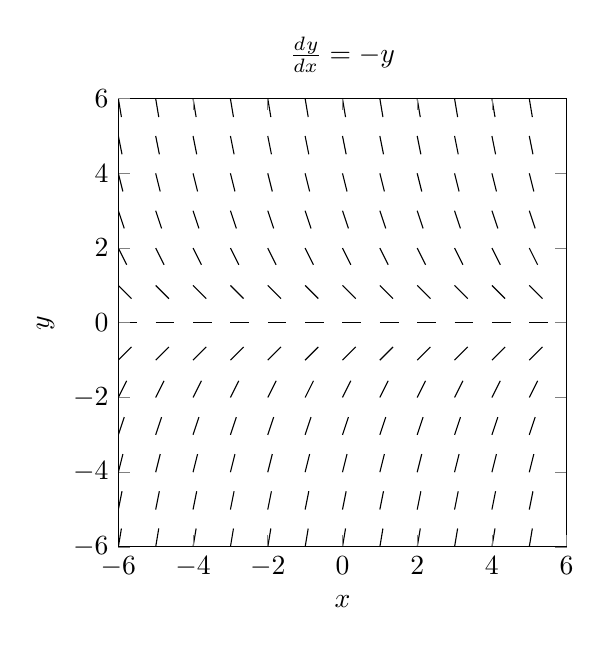
\begin{tikzpicture}
    \begin{axis}[
        xmin = -6, xmax = 6,
        ymin = -6, ymax = 6,
        zmin = 0, zmax = 1,
        axis equal image,
        view = {0}{90},
        title = {$\der{y}{x} = -y$},
        xlabel = {$x$},
        ylabel = {$y$},
    ]
    \addplot3[
        quiver = {
            u = {1/sqrt(1+y^2)},
            v = {-y/sqrt(1+y^2)},
            scale arrows = 0.5,
        },
        samples = 13,
        domain = -6:6,
        domain y = -6:6,
    ] {0};
    \end{axis}
\end{tikzpicture}

$\der{y}{x}$ is negative above the x-axis and positive below it,
so solutions will tend towards $y=0$ as $x \to \infty$.
\newpage
\subsection*{Section 2.2}
\textbf{Problem 3}
Is this equation separable? 
\[
    \der{s}{t} = t\ln(s^{2t}) + 8t^2
\]
\solution
It is separable and can be written as 
\[
    \frac{1}{\ln(s^2)+8}\,ds = t^2 \,dt
\]
\textbf{Problem 5}
Is this equation separable?
\[
    (xy^2 + 3y^2)dy - 2xdx = 0
\]
\solution 
It is separable and can be written as 
\[
    y^2 \,dy = \frac{2x}{x+3} \,dx
\]
\textbf{Problem 9}
Solve the equation
\[
    \der{x}{t} = \frac{t}{xe^{t+2x}}
\]
\solution 
Separating the equation yields 
\begin{align*}
    \der{x}{t} = \frac{t}{xe^{t+2x}}
    &\implies (xe^{t+2x})\der{x}{t} = t \\
    &\implies (xe^{2x}) \,dx = te^{-t} \,dt \\
    &\implies \int (xe^{2x}) \,dx = \int te^{-t} \,dt \\
    &\implies \frac{1}{2}xe^{2x} - \int \frac{1}{2}e^{2x} \,dx =
              -te^{-t} - \int -e^{-t} \,dt \\
    &\implies \frac{1}{2}xe^{2x} - \frac{1}{4}e^{2x} = -te^{-t} - e^{-t} + C \\
    &\implies e^{2x}(2x-1) + 4e^{-t}(t+1) = C
\end{align*}
$\frac{1}{xe^{2x}} \neq 0$, so there are no constant solutions. \\
\textbf{Problem 11}
Solve the equation 
\[
    x\der{v}{x} = \frac{1-4v^2}{3v}
\]
\solution 
Separating the equation yields 
\begin{align*}
    x\der{v}{x} = \frac{1-4v^2}{3v}
    &\implies \frac{3v}{1-4v^2} \,dv = \frac{1}{x} \,dx \\
    &\implies \int 3v(1-4v^2)\inv \,dv = \int \frac{1}{x} \,dx \\
    &\implies -\frac{3}{8}\ln(1-4v^2) = \ln x + C \\
    &\implies 1-4v^2 = Cx^{\frac{8}{3}} \\
    &\implies v = \pm \frac{\sqrt{1-Cx^{\frac{8}{3}}}}{2}
\end{align*}
$\frac{1-4v^2}{3v} = 0$ at $v=\frac{1}{2}$, which is a constant solution. \\
\textbf{Problem 12}
Solve the equation 
\[
    \der{y}{x} = \frac{\sec^2 y}{1+x^2}
\]
\solution 
Separating the equation yields 
\begin{align*}
    \der{y}{x} = \frac{\sec^2 y}{1+x^2}
    &\implies \cos^2 y \,dy = \frac{1}{1+x^2} \,dx \\
    &\implies \int \frac{1 + \cos 2y}{2} \,dy = \int \frac{1}{1+x^2} \,dx \\
    &\implies  \frac{1}{2}y + \frac{1}{4}\sin 2y = \tan\inv x  + C\\ 
\end{align*}
$\sec^2 y \neq 0$, so there are no constant solutions. \\
\textbf{Problem 18}
Solve $y' = x^3(1-y)$ with $y(0) = 3$ \\
\solution 
Separating the equation yields 
\begin{align*}
    y' = x^3(1-y)
    &\implies \frac{1}{1-y} \,dy = x^3 \,dx \\
    &\implies -\ln(y) = \frac{1}{4}x^4 + C \\
    &\implies y = e^{-\frac{1}{4}x^4 + C}
\end{align*}
Pluggin in the initial value yields 
\[
    3 = e^{C} \implies C = \ln(3)
\]
Therefore, the solution is 
\[
    y = e^{-\frac{1}{4}x^4 + \ln(3)}
\]
\textbf{Problem 20}
Solve the equation at $y(1) = 1$
\[
    x^2 \der{y}{x} = \frac{4x^2-x-2}{(x+1)(y+1)}
\]
\solution 
Separating the equation yields 
\begin{align*}
    x^2 \der{y}{x} = \frac{4x^2-x-2}{(x+1)(y+1)} 
    &\implies (y+1) \,dy = \frac{4x^2-x-2}{x^2(x+1)} \,dx \\
    &\implies \int y+1 \,dy 
        = \int -\frac{2}{x^2} + \frac{3}{x+1} + \frac{1}{x} \,dx\\
    &\implies \frac{1}{2}y^2 + y 
        = \frac{2}{x} + 3\ln(x+1) + \ln(x) + C \\
\end{align*}
Plugging in the initial value yields
\[
    \frac{3}{2} = 2 + 3\ln(2) + C 
    \implies C = -\frac{1}{2} - 3\ln(2)
\]
Therefore the implicit solution is 
\[
    \frac{1}{2}y^2 + y 
    = \frac{2}{x} + 3\ln(x+1) + \ln(x) -\frac{1}{2} - 3\ln(2)
\]
\textbf{Problem 22}
Solve the equation at $y(0) = 2$
\[
    x^2 dx + 2y dy = 0
\]
\solution 
Separating the equation yields 
\begin{align*}
    x^2 dx + 2y dy = 0
    &\implies \int 2y dy = \int -x^2 dx \\
    &\implies y^2 = -\frac{1}{3} x^3 + C
\end{align*}
Plugging in the initial value gives
\[
    4 = 0 + C \implies C = 4
\]
Therefore the implicit solution is 
\[
    y^2 = -\frac{1}{3} x^3 + 4
\]
\textbf{Problem 26}
Solve the equation at $y(0) = 1$
\[
    \sqrt{y} dx + (1+x) dy = 0
\]
\solution 
Separating the equation yields 
\begin{align*}
    \sqrt{y} dx + (1+x) dy = 0
    &\implies \int y^{-\frac{1}{2}} dy = \int -\frac{1}{1+x} dx \\
    &\implies 2\sqrt{y} = -\ln(1+x) + C \\
    &\implies y  = \frac{(\ln(x+1) + C)^2}{4}
\end{align*}
Plugging in the initial value gives 
\[
    1 = \frac{C^2}{4} \implies C = 2
\]
Therefore the solution is 
\[
    y  = \frac{(-\ln(x+1) + 2)^2}{4}
\]
\textbf{Problem 30}
\begin{enumerate}
    \item Separate $\der{y}{x} = (x-3)(y+1)^{\frac{2}{3}}$
    \item Show that $y=-1$ satisfies the original equation 
    \item Show that there is no choice of $C$ that will yield $y=-1$.
\end{enumerate}
\solution 
\begin{enumerate}
    \item Separating yields 
        \begin{align*}
            \der{y}{x} = (x-3)(y+1)^{\frac{2}{3}}
            &\implies \int (y+1)^{-\frac{2}{3}} \,dy = \int (x-3) \,dx \\
            &\implies 3(y+1)^\frac{1}{3} = \frac{1}{2}x^2-3x + C \,dx \\ 
            &\implies y = -1 + (\frac{x^2}{6}-x+C)^3
        \end{align*}
    \item At $y=-1$, $\der{y}{x} = (x-3)\cdot 0 = 0$, 
        which is true for constants.
    \item For $y=1$, $(\frac{x^2}{6}-x+C)^3 = 0$ has to be true for all $x$,
        but this is not the case.
\end{enumerate}




\end{document} 
